%%%%%%%%%%%%%%%%%%%%%%%%%%%%%%%%%%%%%%%%%%%%%%%%%%%%%%%%%%%%%%%%%%%%%%%%
% Beamer Presentation - LaTeX - Template Version 1.0 (10/11/12)
% This template has been downloaded from: http://www.LaTeXTemplates.com
% License: % CC BY-NC-SA 3.0 (http://creativecommons.org/)
% Modified by Rahmat M. Samik-Ibrahim

% REV417: Sun 28 Jan 2024 16:00
% REV395: Sun 11 Sep 2022 22:00
% REV386: Thu 28 Jul 2022 13:00
% REV378: Mon 11 Apr 2022 10:00
% REV363: Mon 20 Dec 2021 15:00
% STARTX: Wed 14 Sep 2016 10:00
%%%%%%%%%%%%%%%%%%%%%%%%%%%%%%%%%%%%%%%%%%%%%%%%%%%%%%%%%%%%%%%%%%%%%%%%%

% PACKAGES AND THEMES 
\documentclass[aspectratio=169, xcolor=table, notheorems, hyperref={pdfpagelabels=false}]{beamer}
%%%%%%%%%%%%%%%%%%%%%%%%%%%%%%%%%%%%%%%%%%%%%%%%%%%%%%%%%%%%%%%%%%%%%%%%
% Beamer Presentation - LaTeX - Template Version 1.0 (10/11/12)
% This template has been downloaded from: http://www.LaTeXTemplates.com
% License: % CC BY-NC-SA 3.0 (http://creativecommons.org/)
% Modified by Rahmat M. Samik-Ibrahim
% REV419: Wed 24 Jul 2024 17:00
% REV383: Tue 12 Jul 2022 10:00
% REV316: Wed 14 Jul 2021 13:00
% REV198: Wed 13 Mar 2019 16:00
% REV005: Mon  2 Oct 2017 14:00
% STARTX: Thu 25 Aug 2016 14:00
%%%%%%%%%%%%%%%%%%%%%%%%%%%%%%%%%%%%%%%%%%%%%%%%%%%%%%%%%%%%%%%%%%%%%%%%%

%% ZCZC NNNN
\newtheorem{example}{Example}

%%%%%%%%%%%%%%%%%%%%%%%%%%%%%%%%%%%%%%%%%%%%%%%%%%%%%%%%%%%%%%%%%%%%%%%%%

\let\Tiny=\tiny
\mode<presentation> {
% The Beamer class comes with a number of default slide themes
% which change the colors and layouts of slides. Below this is a list
% of all the themes, uncomment each in turn to see what they look like.
%\usetheme{Boadilla}
\usetheme{Madrid}
% ZCZC %%%%%%%%%%%%%%%%%%%%%%%%%%%%%%%%%%%%%%%%%%%%%%%%%%%%%%%%%%%%%%%%%%
% \usetheme{default} \usetheme{AnnArbor} \usetheme{Antibes} \usetheme{Bergen}
% \usetheme{Berkeley} \usetheme{Berlin} \usetheme{CambridgeUS} 
% \usetheme{Copenhagen} \usetheme{Darmstadt} \usetheme{Dresden}
% \usetheme{Frankfurt} \usetheme{Goettingen} \usetheme{Hannover}
% \usetheme{Ilmenau} \usetheme{JuanLesPins} \usetheme{Luebeck}
% \usetheme{Malmoe} \usetheme{Marburg} \usetheme{Montpellier}
% \usetheme{PaloAlto} \usetheme{Pittsburgh} \usetheme{Rochester}
% \usetheme{Singapore} \usetheme{Szeged} \usetheme{Warsaw}
% NNNN %%%%%%%%%%%%%%%%%%%%%%%%%%%%%%%%%%%%%%%%%%%%%%%%%%%%%%%%%%%%%%%%%%
% As well as themes, the Beamer class has a number of color themes
% for any slide theme. Uncomment each of these in turn to see how it
% changes the colors of your current slide theme.
%\usecolortheme{orchid}
%\usecolortheme{rose}
%\usecolortheme{seagull}
%\usecolortheme{seahorse}
\usecolortheme{whale}
% ZCZC %%%%%%%%%%%%%%%%%%%%%%%%%%%%%%%%%%%%%%%%%%%%%%%%%%%%%%%%%%%%%%%%%%
%\usecolortheme{albatross} \usecolortheme{beaver} \usecolortheme{beetle}
%\usecolortheme{crane} \usecolortheme{dolphin} \usecolortheme{dove}
%\usecolortheme{fly} \usecolortheme{lily} \usecolortheme{wolverine}
% NNNN %%%%%%%%%%%%%%%%%%%%%%%%%%%%%%%%%%%%%%%%%%%%%%%%%%%%%%%%%%%%%%%%%%
% To remove the footer line in all slides uncomment this line
%\setbeamertemplate{footline} 
% To replace the footer line in all slides uncomment this line
%\setbeamertemplate{footline}[page number] 
% To remove the navigation symbols from the bottom uncomment this line
\setbeamertemplate{navigation symbols}{} 
}

\usepackage{array}       % ZCZC
\usepackage{amssymb}     % ZCZC
\usepackage{bold-extra}  % ZCZC
\usepackage{booktabs}    % Allows \toprule, \midrule and \bottomrule in tables
\usepackage{caption}
\usepackage[T1]{fontenc} % ZCZC << >>
\usepackage{graphicx}    % Allows including images
\usepackage{listings}    % listing
\usepackage{lmodern}     % ZCZC
\usepackage{perpage}     % reset footnote per page
\usepackage{geometry}    % ZCZC
\usepackage{adjustbox}   % ZCZC
\usepackage{multicol}    % ZCZC
\usepackage{multirow}    % ZCZC
\usepackage{pgf-pie}     % ZCZC pie chart

% \definecolor{links}{HTML}{2A1B81}
\definecolor{links}{HTML}{0011FF}
\hypersetup{colorlinks,linkcolor=,urlcolor=links}

% \usepackage{xcolor}
% \usepackage[colorlinks = true,
%             linkcolor = blue,
%             urlcolor  = blue,
%             citecolor = blue,
%             anchorcolor = blue]{hyperref}

\captionsetup[table]{name=Tabel}
\makeatletter
\def\input@path{{src/}}
\makeatother
\graphicspath{{src/}}      % src directory
\MakePerPage{footnote}     % reset page

% NNNN %%%%%%%%%%%%%%%%%%%%%%%%%%%%%%%%%%%%%%%%%%%%%%%%%%%%%%%%%%%%%%%%%%

%% % XXXXXXXXXXXXXXXXXXXXXXXXXXXXXXXXXXXXXXXXXXXXXXXXXXXXXXXXXXXXXXXXXXXXXXXXXX
%% % The short title appears at the bottom of every slide, 
%% % the full title is only on the title page
%% \title[Judul Pendek]{Judul Panjang dan Lengkap} 
%% \author{Cecak bin Kadal}
%% \institute[UILA]
%% {
%% University of Indonesia at Lenteng Agung \\ 
%% \medskip
%% \textit{cecak@binKadal.com}
%% }
%% \date{REV00 24-Aug-2016}
%% % \date{\today}
%% 

%% % XXXXXXXXXXXXXXXXXXXXXXXXXXXXXXXXXXXXXXXXXXXXXXXXXXXXXXXXXXXXXXXXXXXXXXXXXX
%% \begin{document}
%% \section{Judul}
%% \begin{frame}
%% \titlepage
%% \end{frame}
%% 
%% % XXXXXXXXXXXXXXXXXXXXXXXXXXXXXXXXXXXXXXXXXXXXXXXXXXXXXXXXXXXXXXXXXXXXXXXXXX
%% \section{Agenda}
%% \begin{frame}
%% \frametitle{Agenda}
%% % Throughout your presentation, if you choose to use \section{} and 
%% % \subsection{} commands, these will automatically be printed on 
%% % this slide as an overview of your presentation
%% \tableofcontents 
%% \end{frame}
%% 
%% % XXXXXXXXXXXXXXXXXXXXXXXXXXXXXXXXXXXXXXXXXXXXXXXXXXXXXXXXXXXXXXXXXXXXXXXXXX
%% \section{UUD dan Pancasila}
%% \subsection{UUD}
%% \begin{frame}
%% \frametitle{Pembukaan}
%% Bahwa sesungguhnya kemerdekaan itu ialah hak segala bangsa dan oleh 
%% sebab itu, maka penjajahan diatas dunia harus dihapuskan karena 
%% tidak sesuai dengan perikemanusiaan dan perikeadilan.
%% \\~\\
%% Atas berkat rahmat Allah Yang Maha Kuasa dan dengan didorongkan oleh 
%% keinginan luhur, supaya berkehidupan kebangsaan yang bebas, maka 
%% rakyat Indonesia menyatakan dengan ini kemerdekaannya.
%% \end{frame}
%% 
%% % XXXXXXXXXXXXXXXXXXXXXXXXXXXXXXXXXXXXXXXXXXXXXXXXXXXXXXXXXXXXXXXXXXXXXXXXXX
%% \begin{frame}
%% \frametitle{Alenia Ketiga}
%% Kemudian daripada itu untuk membentuk suatu pemerintah negara Indonesia 
%% yang melindungi segenap bangsa Indonesia dan seluruh tumpah darah Indonesia 
%% dan untuk memajukan kesejahteraan umum, mencerdaskan kehidupan bangsa, dan 
%% ikut melaksanakan ketertiban dunia yang berdasarkan kemerdekaan, perdamaian 
%% abadi dan keadilan sosial, maka disusunlah kemerdekaan kebangsaan Indonesia 
%% itu dalam suatu Undang-Undang Dasar negara Indonesia, yang terbentuk dalam 
%% suatu susunan negara Republik Indonesia yang berkedaulatan rakyat dengan 
%% berdasar kepada:
%% \begin{itemize}
%% \item Ketuhanan Yang Maha Esa,
%% \item kemanusiaan yang adil dan beradab,
%% \item persatuan Indonesia,
%% \item dan kerakyatan yang dipimpin oleh hikmat kebijaksanaan 
%%       dalam permusyawaratan/ perwakilan,
%% \item serta dengan mewujudkan suatu keadilan sosial bagi seluruh rakyat 
%%       Indonesia.
%% \end{itemize}
%% \end{frame}
%% 
%% % XXXXXXXXXXXXXXXXXXXXXXXXXXXXXXXXXXXXXXXXXXXXXXXXXXXXXXXXXXXXXXXXXXXXXXXXXX
%% \subsection{Pancasila}
%% \begin{frame}
%% \frametitle{Tujuh Kunci Pokok}
%% \begin{block}{Pertama - Kedua - Ketiga}
%% Indonesia ialah negara berdasarkan hukum.
%% Sistem konstitusional.
%% Kekuasaan negara tertinggi di tangan MPR.
%% \end{block}
%% 
%% \begin{block}{Keempat - Kelima}
%% Presiden adalah penyelenggara pemerintahan tertinggi di bawah MPR.
%% Adanya pengawasan DPR.
%% \end{block}
%% 
%% \begin{block}{Keenam}
%% Menteri negara adalah pembantu presiden dan tidak bertanggung jawab 
%% kepada DPR.
%% \end{block}
%% 
%% \begin{block}{Ketujuh}
%% Kekuasaan kepala negara tidak tak tebatas.
%% \end{block}
%% 
%% \end{frame}
%% 
%% % XXXXXXXXXXXXXXXXXXXXXXXXXXXXXXXXXXXXXXXXXXXXXXXXXXXXXXXXXXXXXXXXXXXXXXXXXX
%% \section{Rupa-rupa}
%% \subsection{Kolom}
%% \begin{frame}
%% \frametitle{Kolom}
%% % The "c" option specifies centered vertical alignment 
%% % while the "t" option is used for top vertical alignment
%% \begin{columns}[c] 
%% % Left column and width
%% \column{.45\textwidth} 
%% \textbf{Heading}
%% \begin{enumerate}
%% \item Satu-satu
%% \item Dua-dua
%% \item Tiga-tiga
%% \item Satu-dua-tiga
%% \end{enumerate}
%% 
%% % Right column and width
%% \column{.5\textwidth}
%% Satu-satu~\dots{} aku sayang ibu!
%% Dua-dua~\ldots{} juga sayang ayah!
%% Tiga-tiga~\ldots{} sayang adik kakak!
%% Satu-dua-tiga~\ldots{} sayang semuanya!
%% 
%% \end{columns}
%% \end{frame}
%% 
%% % XXXXXXXXXXXXXXXXXXXXXXXXXXXXXXXXXXXXXXXXXXXXXXXXXXXXXXXXXXXXXXXXXXXXXXXXXX
%% \subsection{Tabel}
%% \begin{frame}
%% \frametitle{Tabel}
%% \begin{table}
%% \begin{tabular}{l l l}
%% \toprule
%% \textbf{Nama} & \textbf{NPM} & \textbf{Tanggal Lahir}\\
%% \midrule
%% Cecak bin Kadal & 1234567890 & 1 Jan 2015 \\
%% Aneh bin Ajaib  & 0987654321 & 31 Des 2014 \\
%% \bottomrule
%% \end{tabular}
%% \caption{Keterangan Tabel}
%% \end{table}
%% \end{frame}
%% 
%% % XXXXXXXXXXXXXXXXXXXXXXXXXXXXXXXXXXXXXXXXXXXXXXXXXXXXXXXXXXXXXXXXXXXXXXXXXX
%% \subsection{Teori}
%% \begin{frame}
%% \frametitle{Teori}
%% \begin{theorem}[Teori Satu Batu]
%% $E = mc^2$
%% \end{theorem}
%% \end{frame}
%% 
%% % XXXXXXXXXXXXXXXXXXXXXXXXXXXXXXXXXXXXXXXXXXXXXXXXXXXXXXXXXXXXXXXXXXXXXXXXXX
%% \subsection{Verbatim}
%% % Need to use the fragile option when verbatim is used in the slide
%% \begin{frame}[fragile] 
%% \frametitle{Verbatim}
%% \begin{example}[Teori Satu Batu]
%% \begin{verbatim}
%% \begin{theorem}[Teori Satu Batu]
%% $E = mc^2$
%% \end{theorem}
%% \end{verbatim}
%% \end{example}
%% \end{frame}
%% 
%% % XXXXXXXXXXXXXXXXXXXXXXXXXXXXXXXXXXXXXXXXXXXXXXXXXXXXXXXXXXXXXXXXXXXXXXXXXX
%% \subsection{Gambar}
%% \begin{frame}
%% \frametitle{Gambar}
%% \begin{figure}
%% \includegraphics[width=0.5\linewidth]{2}
%% \caption{Ini Gambar JPG}
%% \end{figure}
%% \end{frame}
%% 
%% % XXXXXXXXXXXXXXXXXXXXXXXXXXXXXXXXXXXXXXXXXXXXXXXXXXXXXXXXXXXXXXXXXXXXXXXXXX
%% \subsection{Rujukan}
%% % Need to use the fragile option when verbatim is used in the slide
%% \begin{frame}[fragile] 
%% \frametitle{Rujukan dan Kutipan}
%% Contoh penggunaan \verb|\cite| ketika mengutip\cite{p1}.
%% Perhatian: Beamer tidak mengerti \verb|\BibTeX|~\ldots
%% \footnotesize{
%%   \begin{thebibliography}{99} 
%%   \bibitem[Smith, 2012]{p1} John Smith (2012)
%%      \newblock Katak dalam Tempurung
%%      \newblock \emph{Jurnal Kelapa dan Amfibi} 12(3), 45 -- 678.
%%   \end{thebibliography}
%% }
%% \end{frame}
%% 
%% % XXXXXXXXXXXXXXXXXXXXXXXXXXXXXXXXXXXXXXXXXXXXXXXXXXXXXXXXXXXXXXXXXXXXXXXXXX
%% \subsection{Selesai}
%% \begin{frame}
%% \Huge{\centerline{Selesai}}
%% \end{frame}
%% 
%% % XXXXXXXXXXXXXXXXXXXXXXXXXXXXXXXXXXXXXXXXXXXXXXXXXXXXXXXXXXXXXXXXXXXXXXXXXX
%% \end{document}

\newcommand{\revision}{%
REV426: Wed 13 Nov 2024 04:00
}
% w! tmptmp
% REV426: Wed 13 Nov 2024 04:00
% REV419: Wed 24 Jul 2024 17:00
% REV409: Tue 08 Aug 2023 12:00
% REV399: Fri 03 Feb 2023 20:00
% REV339: Sat 04 Sep 2021 12:00
% STARTS: Wed 24 Aug 2016 19:00
%%%%%%%%%%%%%%%%%%%%%%%%%%%%%%%%%%%%%
\newcommand{\kopikopi}{\textcopyright{}2016-2024 CBKadal + VauLSMorg}



% XXXXXXXXXXXXXXXXXXXXXXXXXXXXXXXXXXXXXXXXXXXXXXXXXXXXXXXXXXXXXXXXXXXXXXXXXX
% The short title appears at the bottom of every slide, 
% the full title is only on the title page
% \date{\today}
\title[\kopikopi]
{CSGE602055 Operating Systems \\ 
CSF2600505 Sistem Operasi \\
Week 08:
Scheduling + W06/W07}
\author{C. BinKadal}
\institute[SdnBhd]
{
Sendirian Berhad\\
\medskip
\url{https://docOS.vlsm.org/Slides/os08.pdf}
\\ \texttt{Always check for the latest revision!}
}
\date{\revision}

% XXXXXXXXXXXXXXXXXXXXXXXXXXXXXXXXXXXXXXXXXXXXXXXXXXXXXXXXXXXXXXXXXXXXXXXXXX
\begin{document}

\lstset{
basicstyle=\ttfamily\tiny, % \tiny \small \footnotesize 
breakatwhitespace=true,
language=C,
columns=fullflexible,
keepspaces=true,
breaklines=true,
tabsize=3, 
showstringspaces=false,
extendedchars=true}

\section{Start}
\begin{frame}
\titlepage
\end{frame}

% XXXXXXXXXXXXXXXXXXXXXXXXXXXXXXXXXXXXXXXXXXXXXXXXXXXXXXXXXXXXXXXXXXXXXXXXXX

%%%%%%%%%%%%%%%%%%%%%%%%%%%%%%%%%%%%%%%%%%%%%%%%%%%%%%%%%%%%%%%%%%%%%%%%%
% REV418: Tue 30 Jan 2024 22:00
% REV406: Sat 05 Aug 2023 14:00
% REV399: Thu 02 Feb 2023 00:00
% REV369: Mon 14 Feb 2022 09:00
% REV328: Sat 14 Aug 2021 06:00
% STARTX: Wed 14 Sep 2016 10:00
%%%%%%%%%%%%%%%%%%%%%%%%%%%%%%%%%%%%%%%%%%%%%%%%%%%%%%%%%%%%%%%%%%%%%%%%%

\begin{frame}[fragile]
\section{OS241 Schedule}
\frametitle{OS241\footnote{%
) This information will be on \textbf{EVERY} page two (2) of this course material.}): 
Operating Systems Schedule 2023 - 2}

\vspace{5pt}

\scalebox{0.99}{%
\begin{tabular}{|c|c|l|l|}
\hline
\textbf{Week} & 
\textbf{Topic}\footnote{%
) For schedule, see \url{https://os.vlsm.org/\#idx02}}) & \textbf{OSC10}\footnote{%
    ) Silberschatz et. al.: \textbf{Operating System Concepts}, $10^{th}$ Edition, 2018.}) \\
\hline
Week 00  & Overview (1), Assignment of Week 00           & Ch. 1, 2      \\
Week 01  & Overview (2), Virtualization \& Scripting     & Ch. 1, 2, 18. \\
Week 02  & Security, Protection, Privacy, \& C-language. & Ch. 16, 17.   \\
Week 03  & File System \& FUSE  & Ch. 13, 14, 15.                        \\
Week 04  & Addressing, Shared Lib, \& Pointer & Ch. 9. \\
Week 05  & Virtual Memory & Ch. 10. \\
\hline
Week 06  & Concurrency: Processes \& Threads & Ch. 3, 4. \\
Week 07  & Synchronization \& Deadlock & Ch. 6, 7, 8. \\
Week 08  & Scheduling + W06/W07 & Ch. 5. \\
Week 09  & Storage, Firmware, Bootloader, \& Systemd & Ch. 11. \\
Week 10  & I/O \& Programming & Ch. 12. \\%
% MidTerm  & 00 XXX 2020 (XX:XX-XX:XX) & MidTerm (UTS) & \cellcolor{red!44} TBA! \\
% Reserved & 00 XXX - 00 XXX 2020 & Q \& A & \\
% Final    & 00 XXX 2020 XX:XX & First Part Final  (UAS tahap I)  & \cellcolor{red!44} This schedule is   \\
% Extra    & NA & No Extra assignment & \cellcolor{red!44} subject to change. \\
\hline
\end{tabular}
}
\end{frame}

\begin{frame}[fragile]
\frametitle{\textbf{STARTING POINT} --- 
{
\definecolor{links}{HTML}{FDEE00}
\hypersetup{colorlinks,linkcolor=,urlcolor=links}
\url{https://os.vlsm.org/}
}
}
\begin{itemize}
\item[$\square$] \textbf{Text Book} ---
                 Any recent/decent OS book. Eg. (\textbf{OSC10}) Silberschatz et. al.: 
                 \textbf{Operating System Concepts}, $10^{th}$ Edition, 2018.
                 (See \url{https://codex.cs.yale.edu/avi/os-book/OS10/}).
\item[$\square$] \textbf{Resources ({\footnotesize \url{https://os.vlsm.org/\#idx03}})}
\begin{itemize}
\item[$\square$] \href{https://scele.cs.ui.ac.id/course/view.php?id=3743}{\textbf{SCELE}} ---
\url{https://scele.cs.ui.ac.id/course/view.php?id=3743}.\\
The enrollment key is \textbf{XXX}.
\item[$\square$] \textbf{Download Slides and Demos from GitHub.com} --- (\url{https://github.com/os2xx/docOS/})\\
                 {\scriptsize%
                 \href{https://docOS.vlsm.org/Slides/os00.pdf}{\texttt{os00.pdf} (W00)},
                 \href{https://docOS.vlsm.org/Slides/os01.pdf}{\texttt{os01.pdf} (W01)},
                 \href{https://docOS.vlsm.org/Slides/os02.pdf}{\texttt{os02.pdf} (W02)},
                 \href{https://docOS.vlsm.org/Slides/os03.pdf}{\texttt{os03.pdf} (W03)},
                 \href{https://docOS.vlsm.org/Slides/os04.pdf}{\texttt{os04.pdf} (W04)},
                 \href{https://docOS.vlsm.org/Slides/os05.pdf}{\texttt{os05.pdf} (W05)},\\
                 \href{https://docOS.vlsm.org/Slides/os06.pdf}{\texttt{os06.pdf} (W06)},
                 \href{https://docOS.vlsm.org/Slides/os07.pdf}{\texttt{os07.pdf} (W07)},
                 \href{https://docOS.vlsm.org/Slides/os08.pdf}{\texttt{os08.pdf} (W08)},
                 \href{https://docOS.vlsm.org/Slides/os09.pdf}{\texttt{os09.pdf} (W09)},
                 \href{https://docOS.vlsm.org/Slides/os10.pdf}{\texttt{os10.pdf} (W10)}.
                 }
\item[$\square$] \textbf{Problems}\\
                 {\scriptsize% 
                 \href{https://rms46.vlsm.org/2/195.pdf}{\texttt{195.pdf} (W00)},
                 \href{https://rms46.vlsm.org/2/196.pdf}{\texttt{196.pdf} (W01)},
                 \href{https://rms46.vlsm.org/2/197.pdf}{\texttt{197.pdf} (W02)},
                 \href{https://rms46.vlsm.org/2/198.pdf}{\texttt{198.pdf} (W03)},
                 \href{https://rms46.vlsm.org/2/199.pdf}{\texttt{199.pdf} (W04)},
                 \href{https://rms46.vlsm.org/2/200.pdf}{\texttt{200.pdf} (W05)},\\
                 \href{https://rms46.vlsm.org/2/201.pdf}{\texttt{201.pdf} (W06)},
                 \href{https://rms46.vlsm.org/2/202.pdf}{\texttt{202.pdf} (W07)},
                 \href{https://rms46.vlsm.org/2/203.pdf}{\texttt{203.pdf} (W08)},
                 \href{https://rms46.vlsm.org/2/204.pdf}{\texttt{204.pdf} (W09)},
                 \href{https://rms46.vlsm.org/2/205.pdf}{\texttt{205.pdf} (W10)}.}
\item[$\square$] \textbf{LFS} --- \url{http://www.linuxfromscratch.org/lfs/view/stable/}
\item[$\square$] \textbf{OSP4DISS} --- \url{https://osp4diss.vlsm.org/}
\item[$\square$] \textbf{This is How Me Do It!} --- \url{https://doit.vlsm.org/}
\begin{itemize}
\item[$\square$] PS: "Me" rhymes better than "I", duh!
\end{itemize}
\end{itemize}
\end{itemize}
\end{frame}



% XXXXXXXXXXXXXXXXXXXXXXXXXXXXXXXXXXXXXXXXXXXXXXXXXXXXXXXXXXXXXXXXXXXXXXXXXX
% Throughout your presentation, if you choose to use \section{} and 
% \subsection{} commands, these will automatically be printed on 
% this slide as an overview of your presentation
\section{Agenda}
\begin{frame}{Outline}
  \frametitle{Agenda}
  \tableofcontents[sections={1-}]
\end{frame}
% \begin{frame}
%    \frametitle{Agenda (2)}
%    \tableofcontents[sections={12-}]
% \end{frame}

% XXXXXXXXXXXXXXXXXXXXXXXXXXXXXXXXXXXXXXXXXXXXXXXXXXXXXXXXXXXXXXXXXXXXXXXXXX

%%%%%%%%%%%%%%%%%%%%%%%%%%%%%%%
% REV412: Tue 22 Aug 2023 14:00
% REV406: Sat 05 Aug 2023 12:00
% REV154: Thu 23 Aug 2018 11:00
% START0: Thu 26 Jul 2018 20:00
%%%%%%%%%%%%%%%%%%%%%%%%%%%%%%%

\section{Week 08}
\begin{frame}[fragile]
\frametitle{Week 08 Scheduling:
Topics\footnote{Source: ACM IEEE CS Curricula}}

\begin{itemize}
\item Preemptive and non-preemptive scheduling 
\item Schedulers and policies
\item Processes and threads
\item Deadlines and real-time issues
\end{itemize}
\end{frame}

\begin{frame}[fragile]
\frametitle{Week 08 Scheduling:
Learning Outcomes\footnote{Source: ACM IEEE CS Curricula}}
\begin{itemize}
\item Compare and contrast the common algorithms used for both preemptive and non-preemptive scheduling of tasks in operating systems, such as priority, performance comparison, and fair-share schemes. [Usage]
\item Describe relationships between scheduling algorithms and application domains. [Familiarity]
\item Discuss the types of processor scheduling such as short-term, medium-term, long-term, and I/O.  [Familiarity]
\item Describe the difference between processes and threads. [Usage]
\item Compare and contrast static and dynamic approaches to real-time scheduling. [Usage]
\item Discuss the need for preemption and deadline scheduling. [Familiarity]
\item Identify ways that the logic embodied in scheduling algorithms are applicable to other domains, such as disk I/O, network scheduling, project scheduling, and problems beyond computing. [Usage]
\end{itemize}

\end{frame}



% XXXXXXXXXXXXXXXXXXXXXXXXXXXXXXXXXXXXXXXXXXXXXXXXXXXXXXXXXXXXXXXXXXXXXXXXXX
\section{OSC10 (Silberschatz) Chapter 5}
\begin{frame}
\frametitle{OSC10 (Silberschatz) Chapter 5}
  \begin{itemize}
  \item OSC10 Chapter 5: CPU Scheduling
  \begin{itemize}
  \item Basic Concepts
  \item Scheduling Criteria
  \item Scheduling Algorithms
  \item Thread Scheduling
  \item Multi-Processor Scheduling
  \item Real-Time CPU Scheduling
  \item Operating Systems Examples
  \item Algorithm Evaluation
  \end{itemize}
  \end{itemize}
  \vfill \null
\end{frame}

% XXXXXXXXXXXXXXXXXXXXXXXXXXXXXXXXXXXXXXXXXXXXXXXXXXXXXXXXXXXXXXXXXXXXXXXXXX
\section{Scheduling}
\begin{frame}
\frametitle{Week 08: Scheduling}
\begin{itemize}
\item Reference: (OSC10-ch05 demo-w08)
\item Scheduling
\begin{itemize}
\item Basic Concepts
\begin{itemize}
\item \textbf{WARNING:} It's just a BURST
\item IO Burst
\item CPU Burst
\item CPU Burst vs. Freq (See next slide)
\end{itemize}
\item Criteria: Utilization, throughput, \{turnaround, waiting,  response\} time.
\item (Burst) Algorithm
\begin{itemize}
\item FCFS, SJF, RR, Priority, Multilevel Queue.
\end{itemize}
\item Preemptive / Non-preemptive (Cooperative) Scheduling
\item I/O Bound / CPU Bound Processes
\end{itemize}
\item Thread Scheduling
\begin{itemize}
\item User-level $\rightarrow$ Process-Contention Scope (PCS): many to many/one.
\item Kernel-level $\rightarrow$ System-Contention Scope (SCS): one to one.
\end{itemize}
\item Standard Linux Scheduling
\begin{itemize}
\item Completely Fair Scheduler (CFS).
\item Real Time Scheduling.
\end{itemize}
\end{itemize}
\end{frame}

% XXXXXXXXXXXXXXXXXXXXXXXXXXXXXXXXXXXXXXXXXXXXXXXXXXXXXXXXXXXXXXXXXXXXXXXXXX
\section{CPU Burst: How Long (When)?}
\begin{frame}
\frametitle{CPU Burst: How Long (When)?}
\begin{figure}
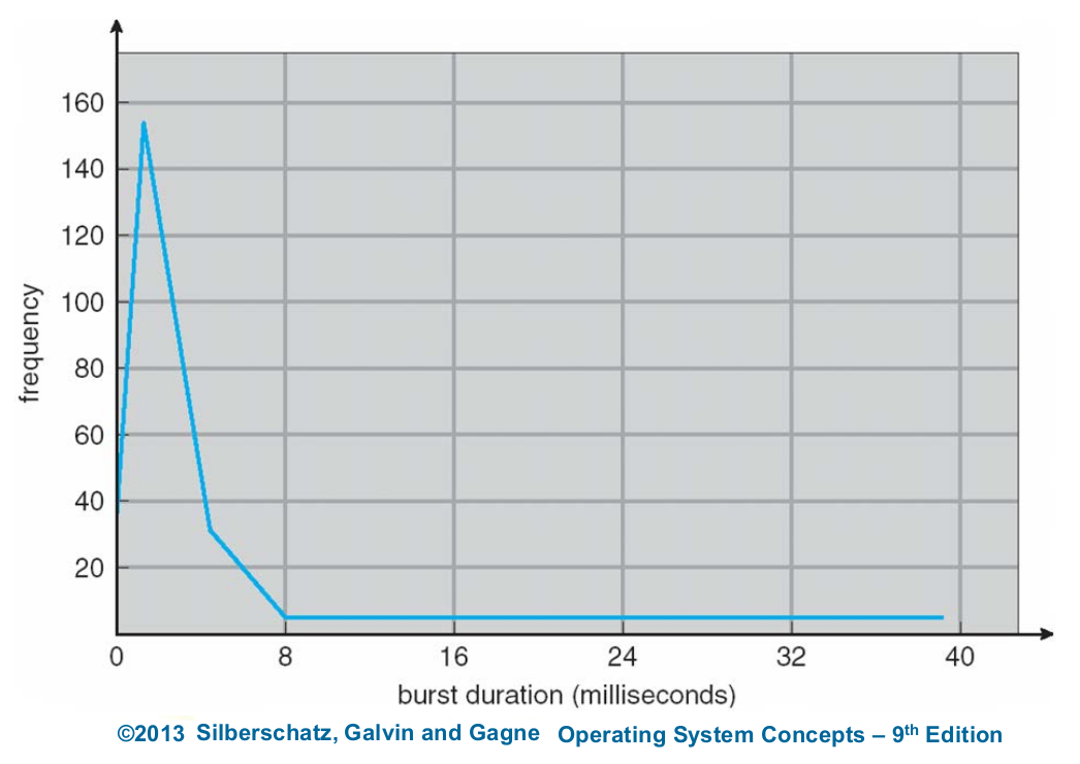
\includegraphics[width=0.60\linewidth]{os08-osc9}
\caption{Burst: Duration vs Frequency}
\end{figure}
\end{frame}

% XXXXXXXXXXXXXXXXXXXXXXXXXXXXXXXXXXXXXXXXXXXXXXXXXXXXXXXXXXXXXXXXXXXXXXXXXX
\section{MultiProcessor Schedulling}
\begin{frame}
\frametitle{MultiProcessor Schedulling}
\begin{itemize}
\item Asymmetric Multiprocessing vs. Symmetric Multiprocessing (SMP).
\item Processor Affinity: soft vs. hard.
\item NUMA: Non-Uniform Memory Access.
\item Load Balancing
\item Multicore Processors
\item Real Time Schedulling: Soft vs. Hard.
\item Big O Notation
\begin{itemize}
\item O(1)
\item O(log N)
\item O(N)
\end{itemize}
\end{itemize}
\end{frame}

% XXXXXXXXXXXXXXXXXXXXXXXXXXXXXXXXXXXXXXXXXXXXXXXXXXXXXXXXXXXXXXXXXXXXXXXXXX
\section{The Two State Model}
\begin{frame}
\frametitle{The Two State Model}
\begin{itemize}
\item CPU State -- I/O State -- CPU State -- \dots
\begin{itemize}
\item n: processes in memory.
\item p: I/O time fraction.
\item $ p^n $: probability n processes waiting for I/O.
\item $ 1 - p^n $: CPU utilization of n processes.
\item $ \left[\frac{\left(1 - p^n\right)}{n}\right] $: CPU utilization of ONE processes.
\end{itemize}
\item Example: $ p = 60 \% \Rightarrow $ \textbf{CPU Utilization Per Process}: $ \left[\frac{1 - \left(60\%\right)^n}{n}\right] $
\\[10pt]
\begin{tabular}{ | c | c | c | c | c | c | }
\hline
\textbf{CPU Utilization}
&
\multicolumn{5}{| c |}{\textbf{Multiprogramming (\%)}} \\
\hline
\textbf{N}
&
\makebox[17pt][c]{\textbf{1}}
&
\makebox[17pt][c]{\textbf{2}}
&
\makebox[17pt][c]{\textbf{3}}
&
\makebox[17pt][c]{\textbf{4}}
&
\makebox[17pt][c]{\textbf{5}}
\\
\hline
\textbf{Per Process} & 40 & 32 & 26 & 21 & 18 \\
\hline
\end{tabular}
\\[10pt]
\begin{itemize}
\item For 5 concurrent processes: \\
If total time is 100 seconds; for each processs, the CPU time will be 18 seconds.
\end{itemize}
\end{itemize}
\begin{table}
\end{table}
\end{frame}

% XXXXXXXXXXXXXXXXXXXXXXXXXXXXXXXXXXXXXXXXXXXXXXXXXXXXXXXXXXXXXXXXXXXXXXXXXX
\end{document}

